\chapter{Decode Stage}
\label{sec:decode_stage}

The Decode Stage is the first DataPath stage and logically it's divided between the DataPath itself and a separated unit called "Decode". The Decode Stage is mainly used to perform the Instruction Decode so identification of instruction type given its \emph{OP\_CODE} and then the dispatch of the operands containted in the instruction towards the DataPath. Meanwhile other side operations are performed like computation of the new PC (given a jump or not), data hazard detection and comparisons.


\section{Instruction Decode}

The most important operation is the Instruction Decode. Here, after the identification of the instruction type, its fields are extracted according to the general instruction structure, as described in Figure \ref{fig:rtype}, Figure \ref{fig:itype} and Figure \ref{fig:jtype}.\\

The Decode is based on the clever shown in Table \ref{table:decode_instr}. The table describes only the signals that go towards the DataPath and not the internal ones.

\begin{table}[H]
    \centering
    \begin{tabularx}{\textwidth}{|l|l|l|l|l|l|X|}
        \hline
        \textbf{Instruction} & INP1 & INP2 & RS1 & RS2 & WS & Note\\
        \hline
        RTYPE & \texttt{0} & \texttt{0} & \texttt{IR[25:21]} & \texttt{IR[20:16]} & \texttt{IR[15:11]} & \\
        \hline
        J & \texttt{0} & \texttt{0} & \texttt{R0} & \texttt{R0} & \texttt{R0} & \\
        \hline
        JAL (CALL) & \texttt{0} & \texttt{PC} & \texttt{R0} & \texttt{R0} & \texttt{R31} & \\
        \hline
        JALR & \texttt{0} & \texttt{PC} & \texttt{IR[25:21]} & \texttt{R0} & \texttt{R31} & \\
        \hline
        TICKTMR & \texttt{0} & \texttt{\emph{i\_TICKTMR}} & \texttt{R0} & \texttt{R0} & \texttt{IR[25:21]} & Destination reg on [25:21]\\
        \hline
        ITYPE & \texttt{0} & \texttt{IR[15:0]} & \texttt{IR[25:21]} & \texttt{IR[20:16]} & \texttt{IR[20:16]} & INP2 Sign Extension iff \emph{UNSIGNED\_ID}\\
        \hline
        LHI & \texttt{IR[15:0]} & \texttt{16} & \texttt{IR[25:21]} & \texttt{IR[20:16]} & \texttt{IR[20:16]} & No Sign Ext\\
        \hline
    \end{tabularx}
    \caption{Instruction Decoding}
    \label{table:decode_instr}
\end{table}

For Jump or Branch instruction, the immediate field doesn't go beyond the decode stage itself. The immediate is a relative value to be summed to the actual PC in case of a taken jump. For Jump-like instructions (J, JAL, CALL) the field is 26 bit long (far jumps) while for other branch instructions the field is 16 bit long (near jumps). In both cases the value is extended to 32 bit with sign because the relative value can be both positive (forward jumps) and negative (backward jumps).

\section{Register File and Windowing}
The general structure of a register file is based on a decoder that takes the selection input (so the address of the desired register) and enables it (using also the enable signal). At this point, an input signal will contain the value to be written. On the other hand, a read signal is used to select among all the registers.\newline\newline
The DLX presented in this document has been enhanced in order to be able to manage subroutine in a transparent manner from the point of view of the user. For this reason, the DLX must be able to handle subroutines, and so the context switching, that consists in saving the
registers content in order to be restored once the procedure has been completed. The straightforward solution is to save into the memory all registers but this is not feasible in terms of delay, since for 32 registers we will need 32 clock cycles; if you image this in a pipeline, this corresponds to a long stall each time a procedure is called.

A windowed register allows to reduce the overhead due to the context switch; the basic idea
is to split the available registers in the physical register file into blocks, called \textit{windows}. We have limited amount of physical registers in the register file, for this reason a finite number of windows are defined. Each window is assigned to a subroutine, so that the procedure can write only on those register. This is transparent from the point of view of the CPU, that sees all registers available. Thus, the physical register file has a wrapper around it with a logic and a Register Management Logic (MML) that allows to perform the translation between the CPU requests to corresponding window for the running procedure.\newline\newline
What if the number of called procedure is larger than the number of available windows? The main
memory is involved only when there are no free windows in the register file. In this case, the oldest allocated window is swapped into the main memory, so that the new one can be allocated. Obviously, once all the recursion chain has been unrolled, the swapped window in the memory must be restored into the register file.
All windows, so each procedure, has 4 blocks of 8 registers each one:
\begin{enumerate}
	\itemsep0sp
	\item \textbf{IN}: the first block is dedicated to the data inherited from the parent routine (OUT);
	\item \textbf{LOCALS}: contains the registers that are dedicated to the procedure;
	\item \textbf{OUT}: is dedicated to the variables to be passed to the child routine, that is the IN of the next sub-procedure
	\item \textbf{GLOBAL}: the last block is common to every windows.
\end{enumerate}
When a procedure is called, the first LOCALS and OUT blocks are allocated from the physical file register and assigned to it (because IN is the OUT of the previous one).

By calling many nested procedures, at some point there will be no free windows; for this reason the oldest is de-allocated from the physical FR and swapped to the main memory, the operation is called \textbf{SPILL}. This it accomplished by using a support pointer, called \textbf{Saved Window Pointer SWP} that stores the point of the spilled data, exactly the end of the LOCALS block (only IN and LOCAL are spilled, the OUT block is not spilled because is the IN of the next sub-procedure). In practice it define the position of the last free cell. Notice that this operation cannot be executed in one clock cycle: each register is spilled once at a clock cycle.\newline\newline
On the other hand, when the last procedure in the chain is finished, the other are unrolled; if some of them have been spilled, a \textbf{FILL} must be executed before the actual execution. This can be achieved by, firstly decrement CWP by 16 and check if now CWP $>>$ SWP.\newline\newline
It's important to notice that the implementation of the entire register file has been implemented in Structural. Is is composed by several components:
\begin{itemize}
	\item \textbf{Decoder}: it is used to generate a single enable signal from a signal on \textbf{NBIT\_ADD} bits; in this way, a register is selected in order to perform a write. The register will check also if a write is requested;
	\item \textbf{Connection matrix}: this block allows to ``highlight" the active windows, the block IN, LOCAL and OUT will be the default destination when writing and reading;
	\item \textbf{Register file}: this block corresponds to the physical registers, composed by rows of Flip-Flops;
	\item \textbf{Select block}: this block is used for the reading, is connected to all the registers and selects, using the read address, the single register to be read;
	\item \textbf{Address generator}: this block is used only when perform a FILL or a SPILL, it generates the address for the registers to be moved from/to the memory. The memory, in this case works exactly like a stack;
	\item \textbf{WRF Control Unit}: A FSM used to manage the address generator when performing a SPILL or a FILL.
\end{itemize}
Additional, but less complex components, have been used in order to manage the CWP and SWP. The complete diagram is available at Figure \ref{figure:wrf_complex}.


\subsection{Decoder}
This block receives as input the \emph{write address} on \textbf{NBIT\_ADD} bits and outputs \(\mathbf{2^{NBIT\_ADD} - 1} \) bits. It has the utility of converting the address of the register at which we need to write into its enable signal. 

The idea is that if the input is \(0b00010\) the output will be \(0b00000000000000000000000000000100\). In fact if the input is decimal 2, it means that we need to write the second register of the \emph{GLOBAL} block. In terms of enable it can be translated by having the bit with index 2 at one. In fact in the output we see that the it with index 2 has value 1, while the others are all 0. 

The output is divided (in the schematic) in order to represent the group of bits. In particular we have that: 
\begin{itemize}
    \item M - 1 DOWNTO 0: bits associated to the \emph{GLOBAL} register
    \item M + N - 1 DOWNTO M: bits associated to the \emph{IN} register
    \item M + 2N - 1 DOWNTO M + N: bits associated to the \emph{LOCAL} register
    \item M + 3N - 1 DOWNTO M + 2N: bits associated to the \emph{OUT} register
\end{itemize}

On the top of the schematic (\autoref{decoder}) we can see an AND logic port between \emph{ENABLE} and \emph{WR} signals. If both \emph{ENABLE} and \emph{WR} are 1, it means that our register need to work. In fact, the output of the dedocer is anded with 1 and so we maintain the value. Otherwise, if one signal between \emph{ENABLE} and \emph{WR} is 0, the output will be 0 and so the AND with the output of the \emph{decoder} will return all 0. 

This signal goes into the \emph{connection matrix}, which is the next block described. 

%% MAKE FONT BIGGER
\begin{figure}[ht]
    \centering
    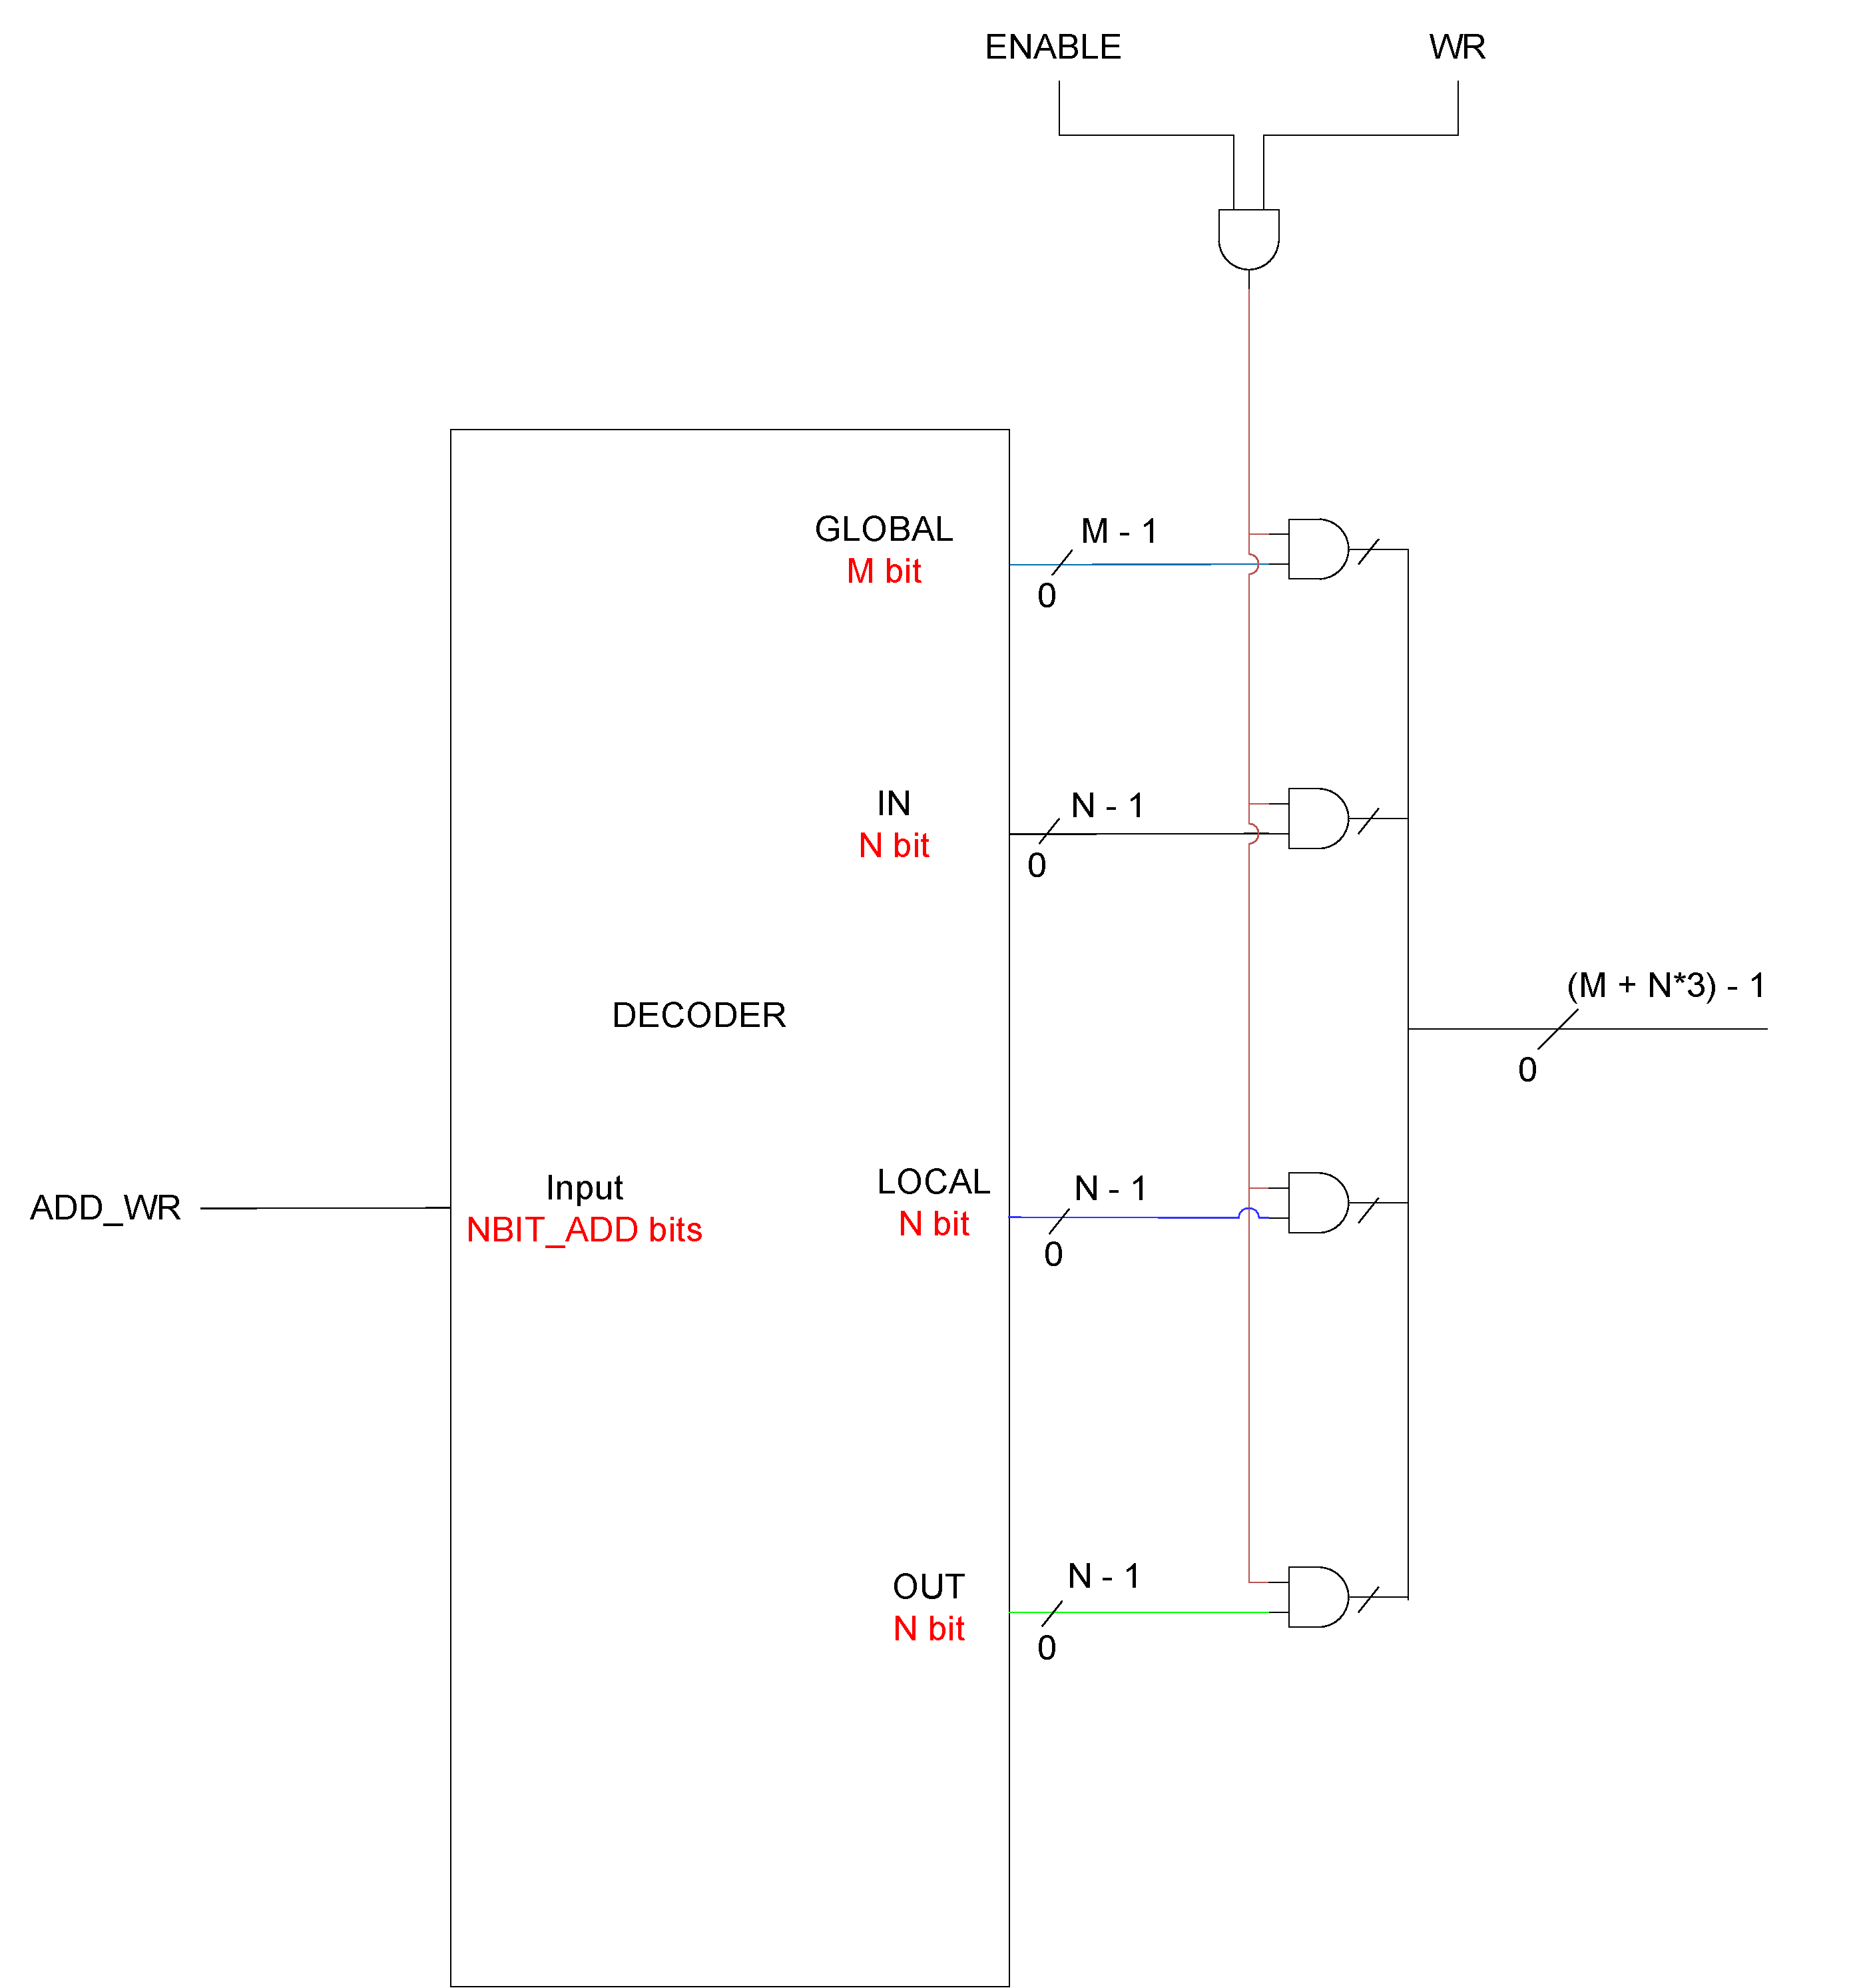
\includegraphics[width=0.7\textwidth]{chapters/4_DecodeStage/images/Decoder.pdf}
    \caption{Schematic of the Decoder}
    \label{decoder}
\end{figure}
%% MAKE FONT BIGGER

\subsection{Connection Matrix}

With the previous block, we generated all our enable signals. The problem is that we have more windows. So how do we decide which window needs to be activated? Here comes the connection matrix. This block receives as inputs the signal coming from the decoder, the current window, the saved window and the address for the pop (fill) operation. The output is a signal that contains the enable signals ready for all the registers of all windows. 

We have a specific structure for each block:
\begin{itemize}
  \item GLOBAL: the global is the simplest, because it is connected directly to the output
  \item IN: for this block we AND the IN bits coming from the decoder with the bit (that is extended) of the related window. For example if we are evaluating the IN of the first window, we will AND the IN bits with the bit 0 of the current window.
  \item OUT: for this block we AND the OUT bits coming from the decoder with the bit (that is extended) of the previous related window. For example if we are evaluating the OUT of the first window, we will AND the OUT bits with the bit 4 of the current window (supposing our window has 5 bits).
  \item LOCAL: for this block we AND the LOCAL bits coming from the decoder with the bit (that is extended) of the related window. For example if we are evaluating the LOCAL of the first window, we will AND the LOCAL bits with the bit 0 of the current window.
\end{itemize}

For the IN and OUT we then an OR between the two outputs (the logic can be seen in the schematic), while for the LOCAL we don't have anything.

In addition to that, the connection matrix also manages the saved window, used for the pop (fill) operation. First we need to invert the addr\_pop, because when we execute the pop operation, we restore data starting from the last one (we are using a STACK).
The addr\_pop\_inverted is composed like this:
\begin{itemize}
  \item 2N - 1 DOWNTO 0: we have the IN bits 
  \item N - 1 DOWNTO 0: we have the LOCAL bits
\end{itemize}

The signal is splitted into two wires and is anded with the saved related saved window pointer. 

In the end, we definitely OR the output of the previously described OR with the output of this AND. This is visible in \autoref{connection_matrix}

\begin{figure}[H]
  \centering
  \addtolength{\leftskip}{-3cm}
  \addtolength{\rightskip}{-3cm}
  \includegraphics[width=1.3\textwidth]{chapters/4_DecodeStage/images/connection_matrix.pdf}
  \caption{Connection matrix}
  \label{connection_matrix}
\end{figure}

\newpage

\subsection{Register File}

The next block is the Register File, that is a sequence of registers. The important thing to notice in our design is how we managed the data that goes into the registers. We have two choices, data\_in and from\_mem. In order to choose we decided to use multiplexers. 
We have a multiplexer for each window. The signal used to drive the multiplexer is the saved window pointer, rotated right by 1 position and anded with the pop signal. In fact, we select from\_mem only when the pop signal is 1, otherwise we need to select data\_in. 
We use the saved window pointer shifted right by 1 because when the saved window pointer is, for example 00010 we need to restore the window 00001. 

Indeed, for dataout there are no multiplexers, because there is no choice. 

\subsection{Select Block}

This block is very simple and straightforward. It receives as input the current window, and the output of the register file (of all windows). The it selects the bit of the IN, LOCAL, OUT of the current window. The interface is shown in \autoref{select_block}.

\begin{figure}[ht]
  \centering
  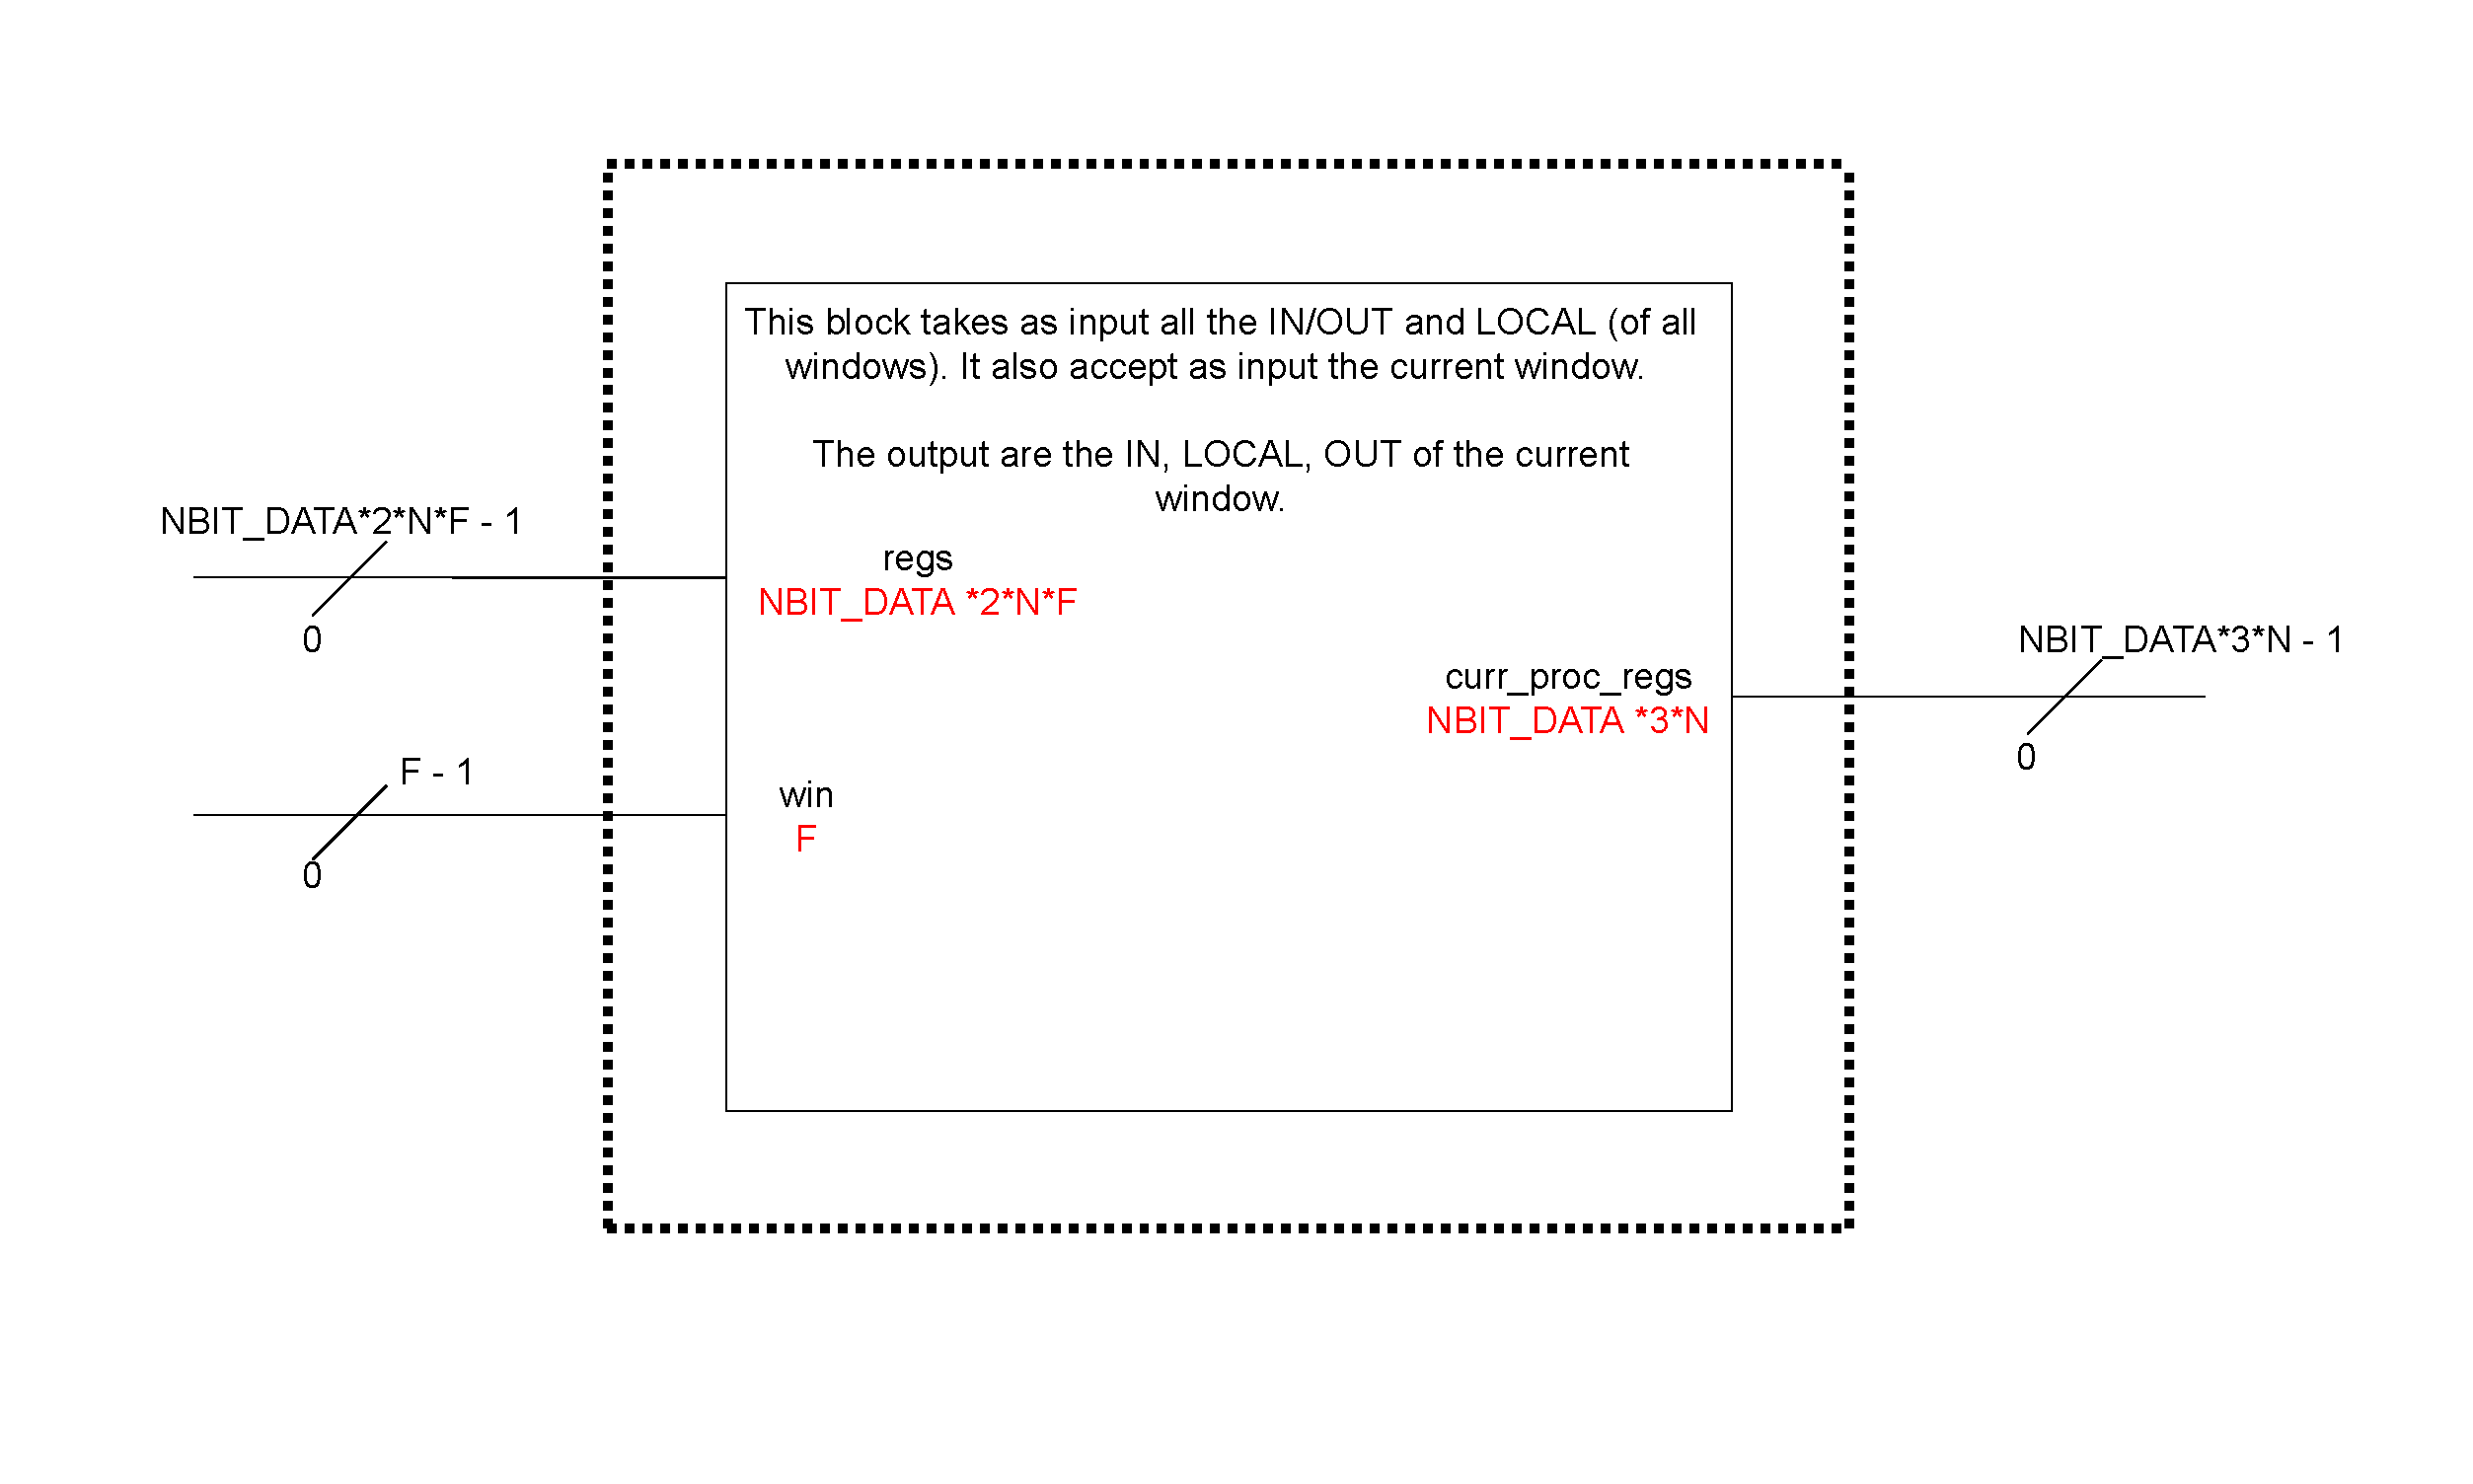
\includegraphics[width=0.9\textwidth]{chapters/4_DecodeStage/images/select_block.pdf}
  \caption{Interface of the select block}
  \label{select_block}
\end{figure}

\subsection{Output Selection}
This is the stage that decide the two output Data1\_Out and Data2\_Out. The design is shown in \autoref{output_choice}.

\begin{figure}[H]
  \centering
  \includegraphics[width=0.8\textwidth]{chapters/4_DecodeStage/images/output_choice.pdf}
  \caption{Design of the output selection}
  \label{output_choice}
\end{figure}

This stage receives the IN, LOCAL, OUT of the current window, thanks to the select block and the GLOBAL. The two addresses, ADD\_RD1 and ADD\_RD2, select the output of the multiplexer which goes into the register, used to respect the timing. The Enable of each register is the and of the ENABLE and the RD signal. The decision was made in order to stop reading when the circuit is not enabled, and so to have a granural and precise control of the circuit.

\subsection{Next Window Calculator}

This block is used to compute the next window, both for the current window and the saved window. The schematic is shown in \autoref{nwin_cal}.

\begin{figure}[H]
  \centering
  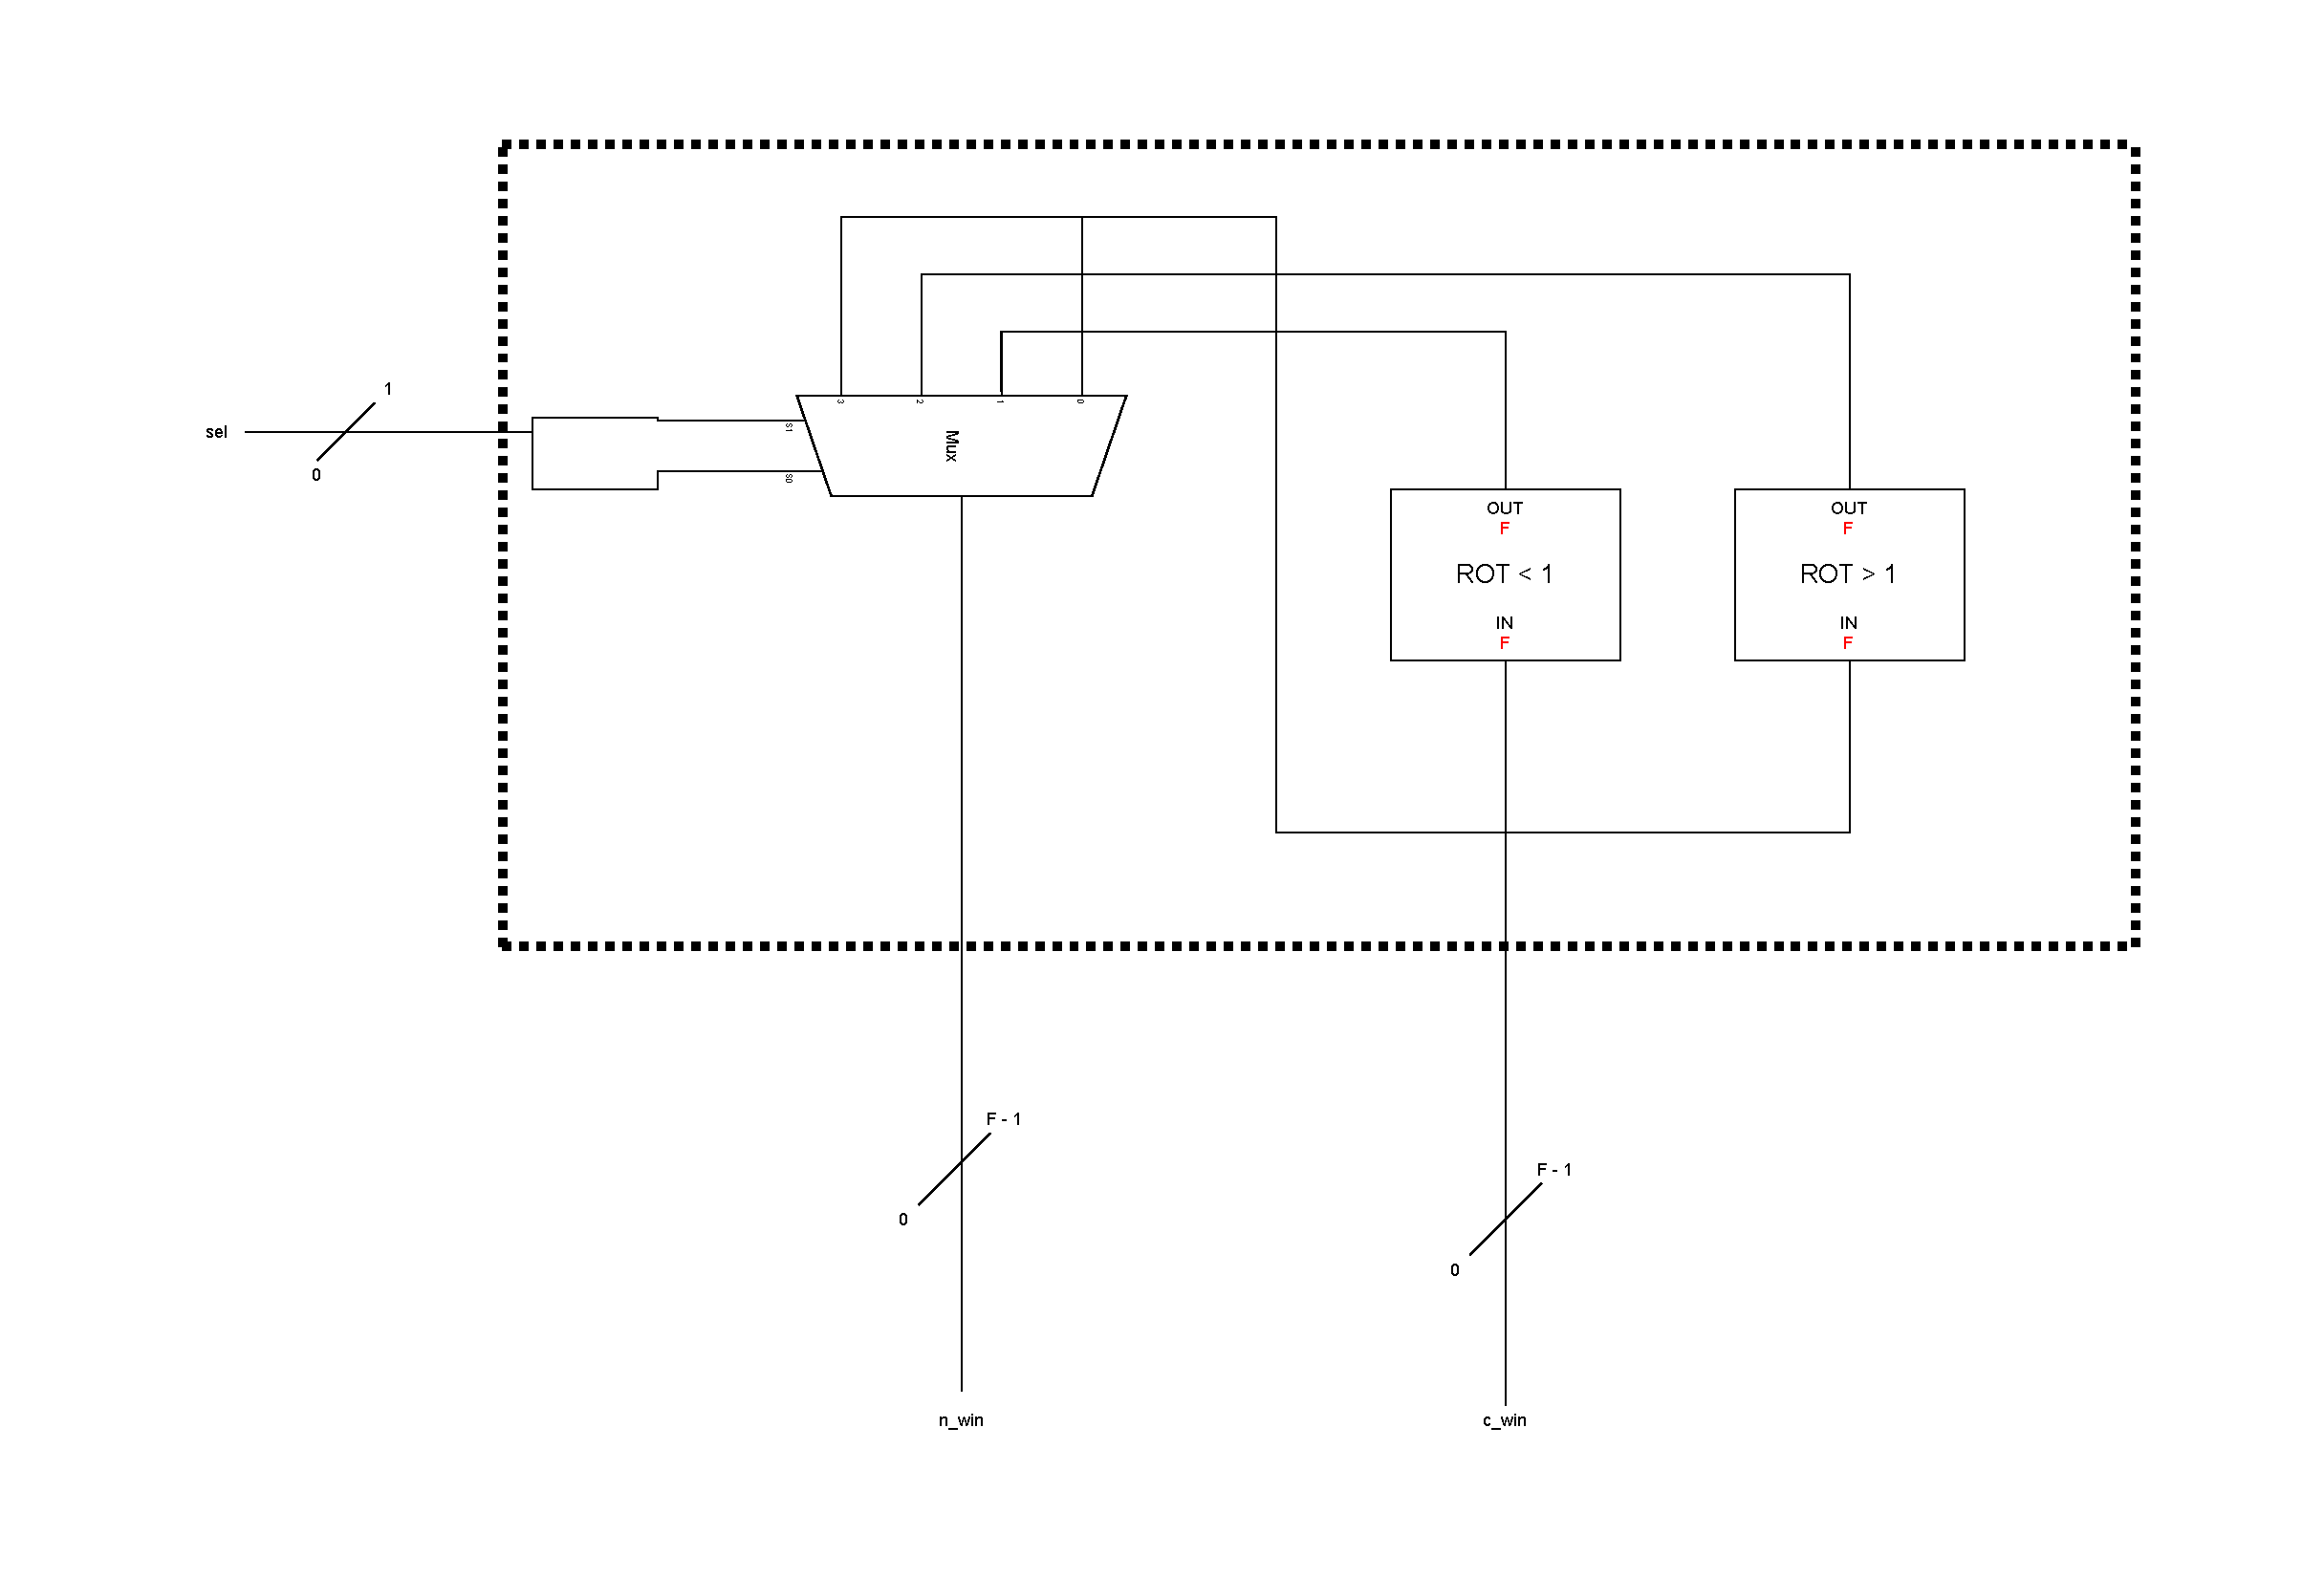
\includegraphics[width=0.9\textwidth]{chapters/4_DecodeStage/images/nwin_cal.pdf}
  \caption{Design of the next window calculator}
  \label{nwin_cal}
\end{figure}

Inside this block there is a logic able to rotate right or left and a multiplexer, that allows to select the correct output based on what the circuit needs. 

\subsection{WRF Control Unit}

An additional element is necessary in order to be able to manage the addresses for the SPILL and FILL procedure, to and from the memory. It has been implemented using a Moore FSM and basically consists in different phases; a starting one that set the memory address to 0 and when the FILL or SPILL input is `1' and the ram is ready, the address is decreased or increased by 4, accordingly to the operation. Refer to figure \ref{wrf_cu}. It's important to say that, if the RAM is not ready the address is keep untouched, so that, when the RAM returns in a ready state, the procedure can continue.


\begin{figure}[ht]
	\centering
	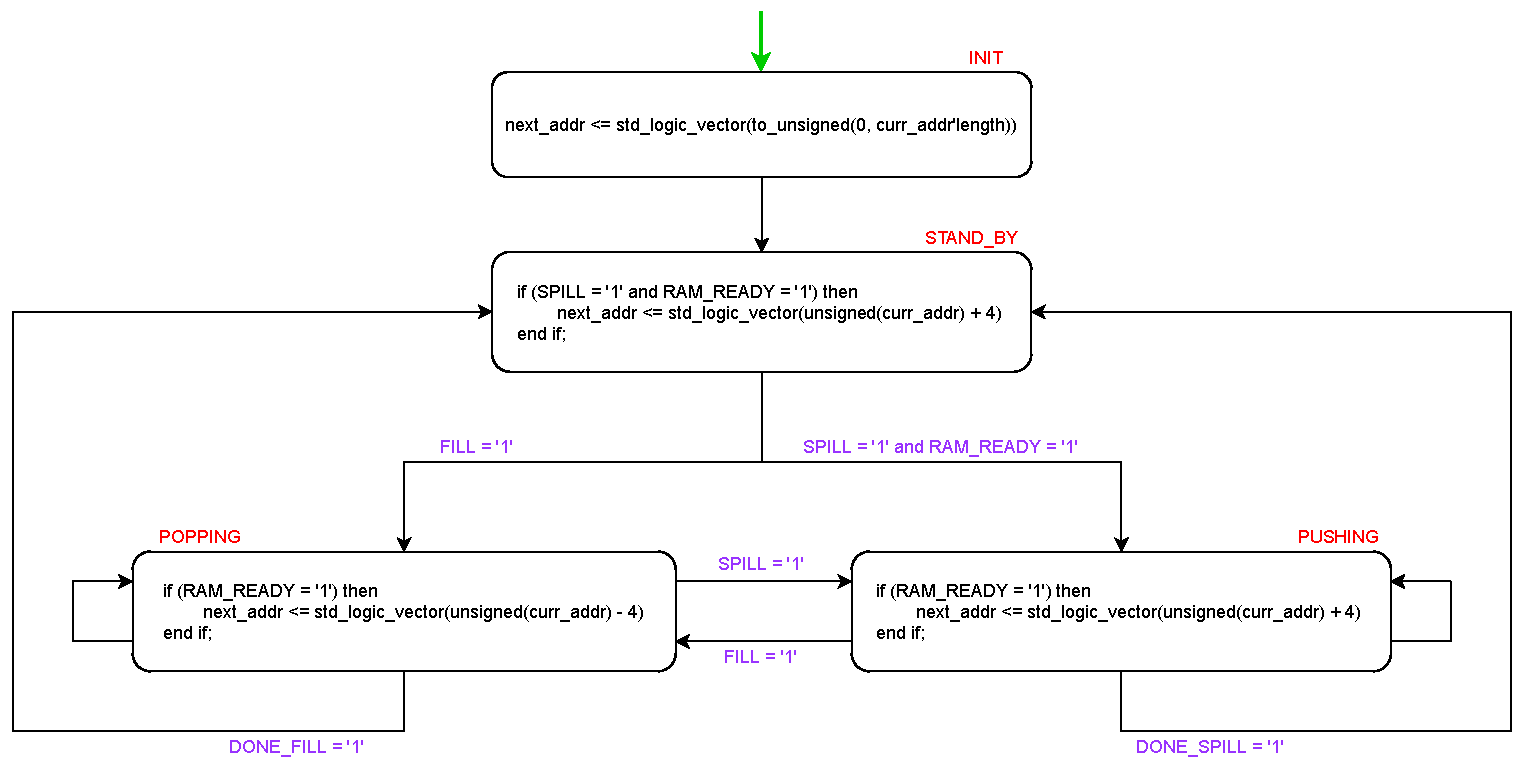
\includegraphics[width=0.8\textwidth]{chapters/4_DecodeStage/images/wRF_CU.pdf}
	\caption{Moore FSM implementation for WRF CU}
	\label{wrf_cu}
\end{figure}

\section{Hazard Control}
To exploit this funciontality the starting point was to understand when to stop the pipeline. Problems may occur in read after write and also when changing window for the CALL and RET procedures. 
The first solution implemented was the use of a table with 32 entry of 1 bit each. When an operation needed to write on a specific register, the bit of the entry related to the register would have been set to 1. When the operation was over, the bit would go back to 0. This solution was perfectly working, but the main problem was scalability and adaptabilty. In fact, if two ore more consecutive operations needed to write on the same register and then another operation need to read that register, the single bit was not enought and it was causing malfunctioning. The problem was that the second operation simply overwrite a 1 on the table. So, when the first operation finish, it set the bit to 0 while the second operation is still writing that register and so the third operation, that is reading that register, could start, but reading a wrong value on the register. 

The solution to this problem was to simply increase the number of bit of each entry of the table. Each time an operation need to write a register it increases the value of the Table (at the specific entry). When the operation finishes, the value is decreased. Thanks to this trick, the example explained before, now works perfectly. 
The chosen number of bits was 3, in order to be able to count 7, that is an higher number compared to the pipeline stages. 

\section{Comparator}
\label{sec:comparator}
The straightforward way to implement a comparator, allows only to check if two operands, \texttt{A} and \texttt{B}, are equals. The solution is sketched at figure \ref{fig:comparator_basic}, that is based on $N$ XNOR, where $N$ is the number of bits of the operands and an AND gate with $N$ inputs.

Even if this solution is extremely compact, it allows to perform only the equality comparison; since this DLX implementation has the ability to perform complex conditional branch instructions (refer to the Instruction section \ref{section:inst_set}) and conditional set instructions (refer to the Set-Like Operations Unit \ref{section:set_link_operations_unit}) we need a more complex solution. In fact, if we need to perform a jump only if \texttt{A} $>$ \texttt{B} (strictly greater) we need to check exactly this precise condition.

\begin{figure}[H]
	\centering
	\begin{minipage}{.5\textwidth}
		\centering
		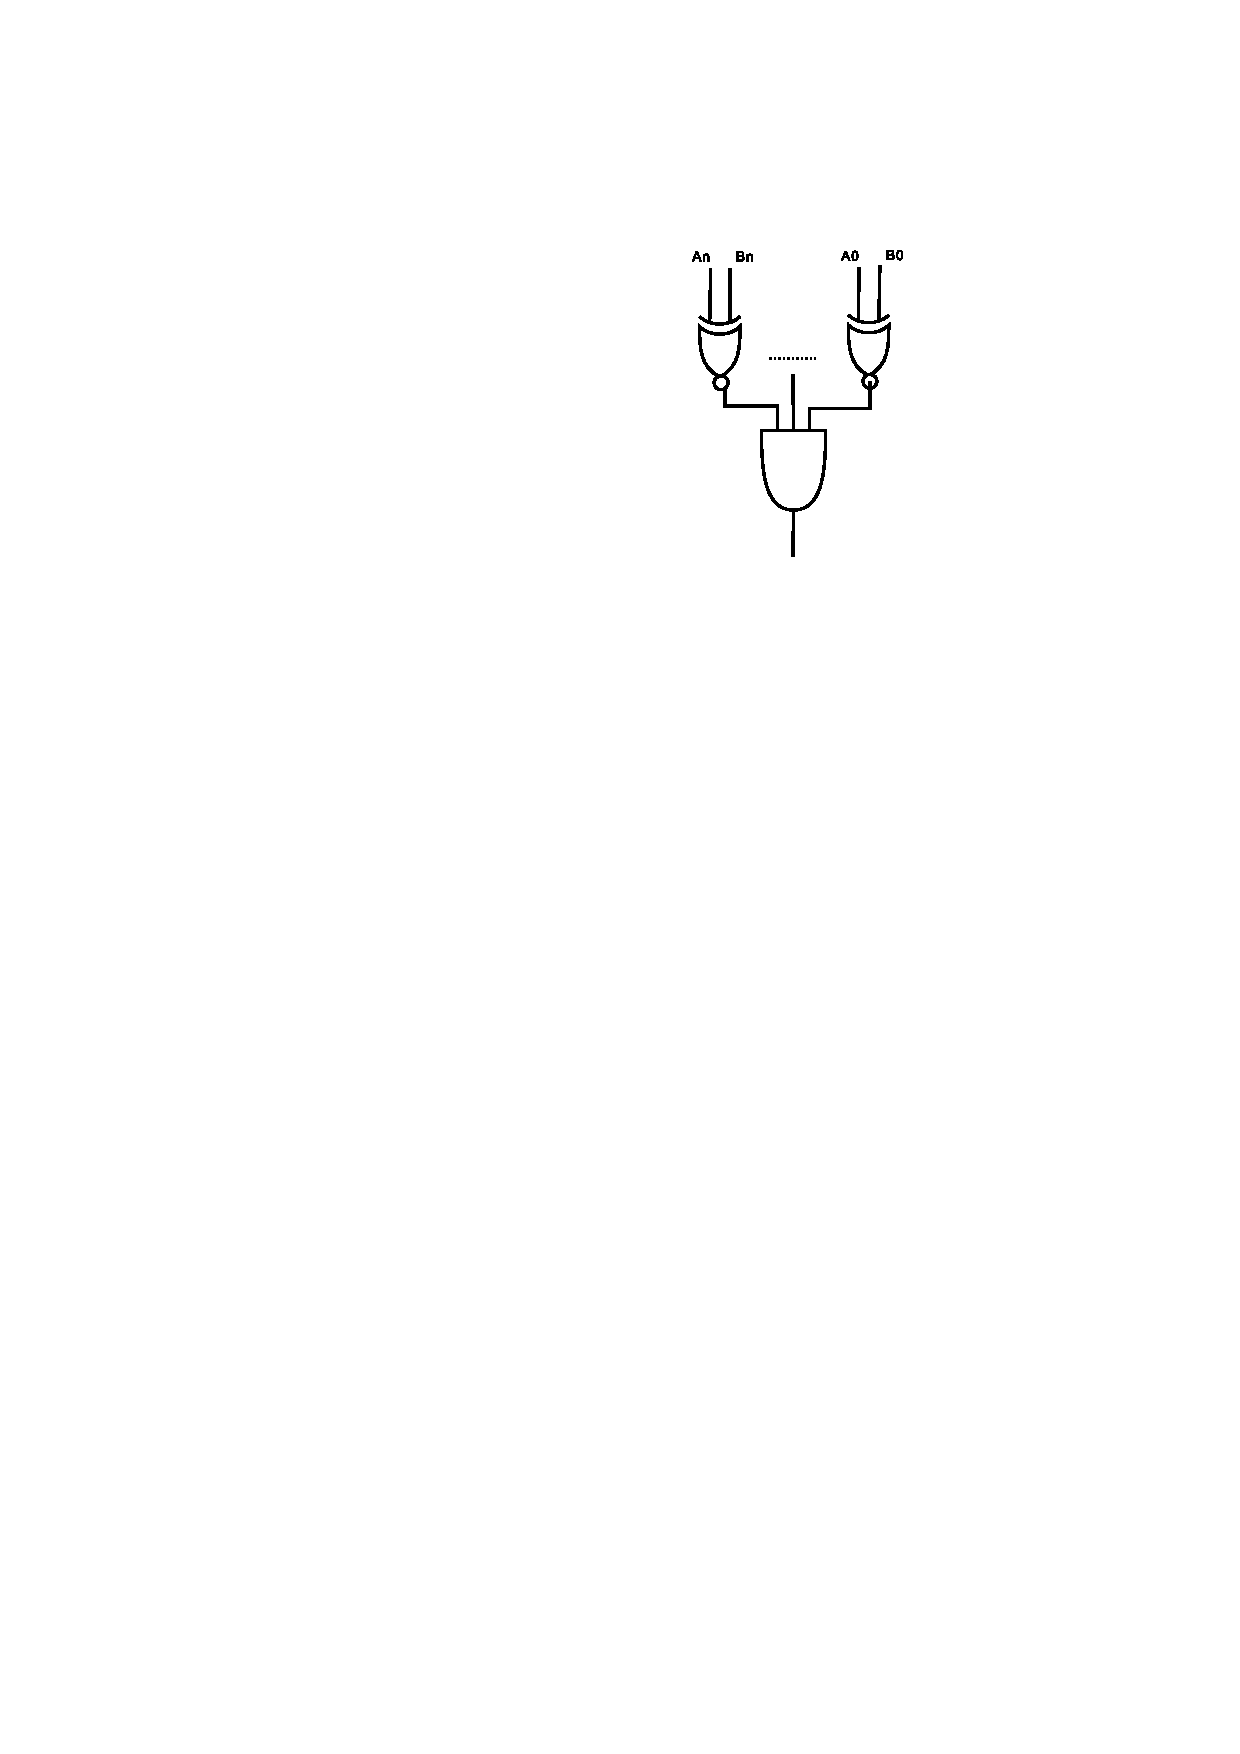
\includegraphics[width=0.55\textwidth]{chapters/4_DecodeStage/images/comparator_basic.pdf}
		\caption{Design of the basic comparator}
		\label{fig:comparator_basic}
	\end{minipage}%
	\begin{minipage}{.5\textwidth}
		\centering
		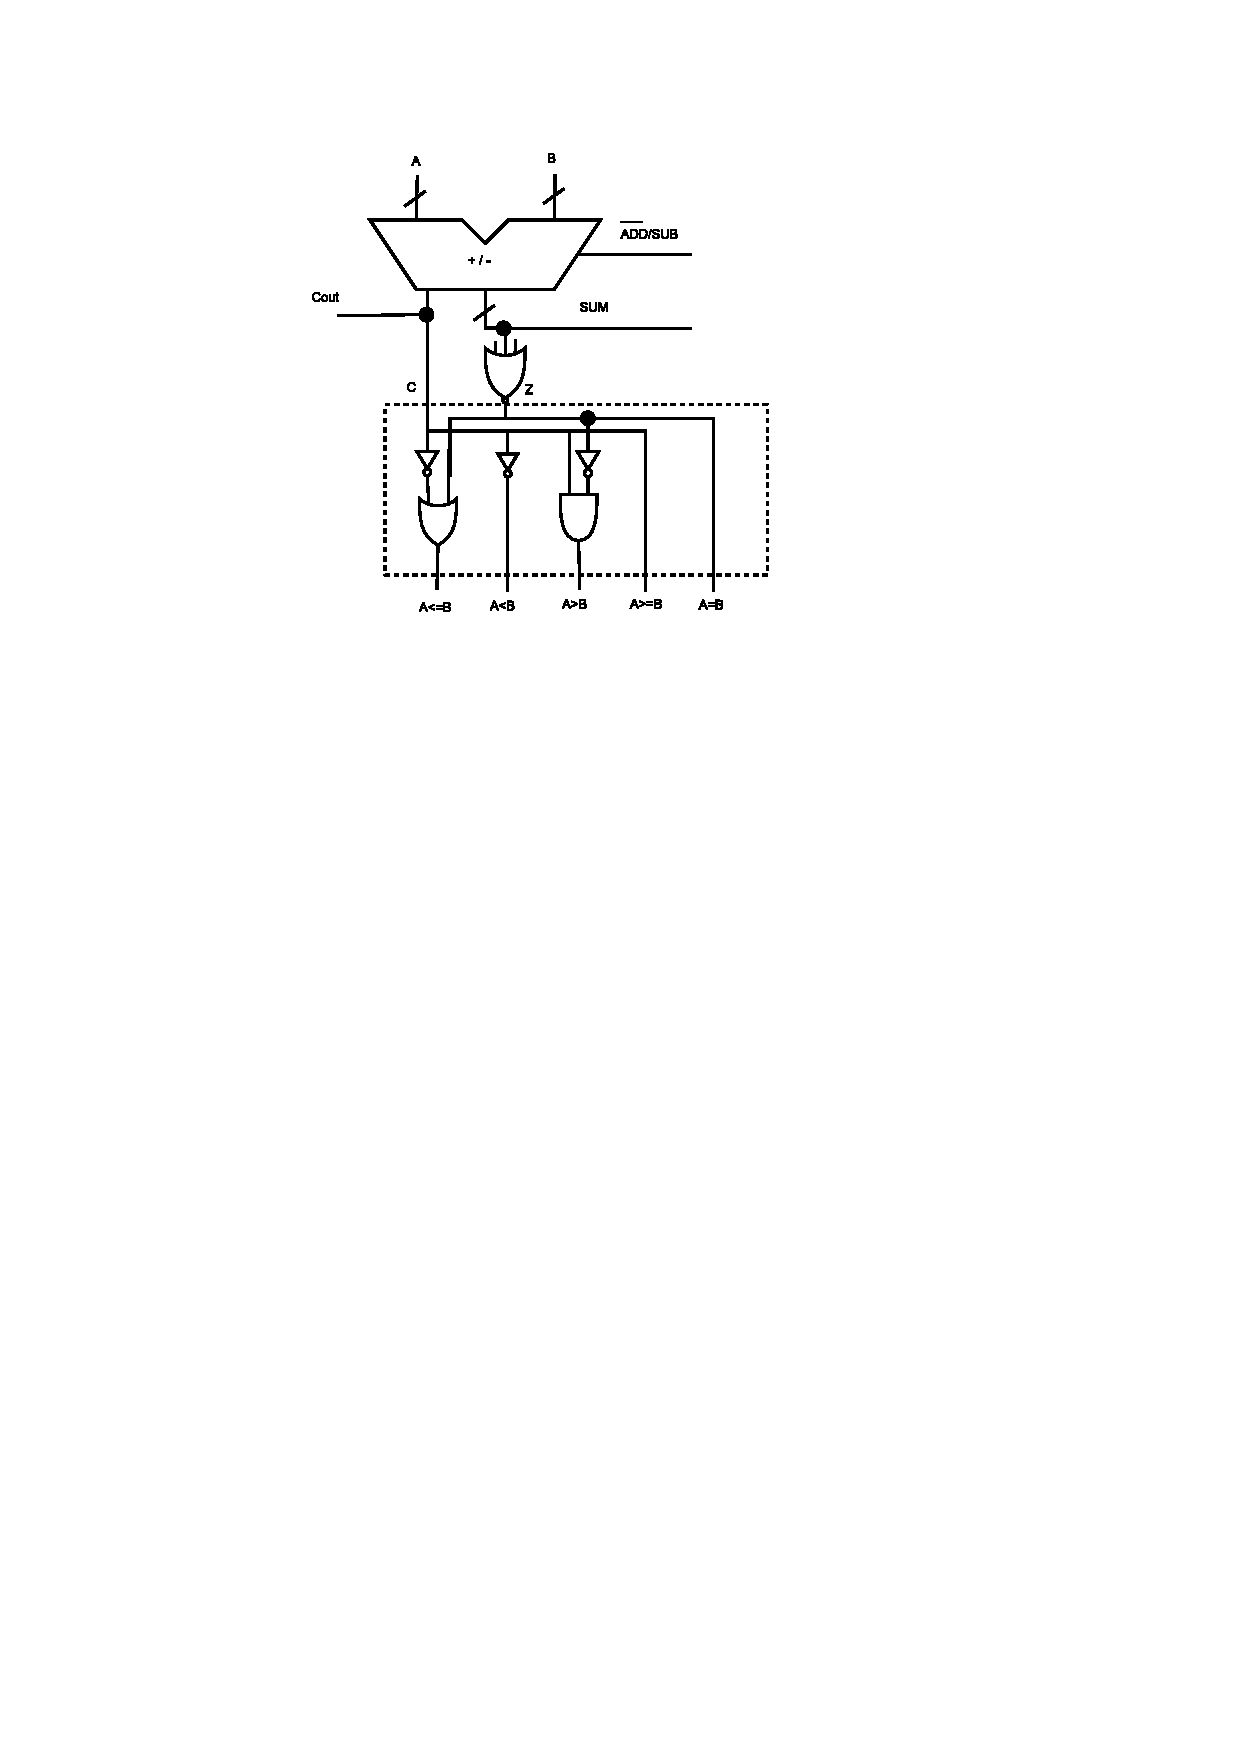
\includegraphics[width=0.7\textwidth]{chapters/4_DecodeStage/images/comparator_advanced.pdf}
		\caption{Design of the advanced comparator}
		\label{comparator_advanced}
	\end{minipage}
\end{figure}

The advance comparator exploits the comparison by performing a subtraction between \texttt{A} and \texttt{B} and then checking the result. This DLX implementation is based on a P4 adder that is able to perform subtraction and then a set of checks, the same that are in the \ref{comparator_advanced} are performed in order to generate the comparison outputs. We can perform the comparisons using this boolean equations, where $C$ is the carry-out and $Z$ is the zero check (all bits of the results are zeros):
\begin{align*}
	A > B &\rightarrow C \cdot \overline{Z}\\
	A \geq B &\rightarrow C\\
	A < B  &\rightarrow \overline{C}\\
	A \leq B &\rightarrow \overline{C} + Z\\
	A = B &\rightarrow Z\\
	A \neq B  &\rightarrow \overline{Z} 
\end{align*}

 In order to avoid to propagate six different signal, the outcomes of the comparisons are encoded into a signal \texttt{LGET} on two bits. The encoded value are the ones in the Table \ref{tab:lget}.
 \begin{multicols}{2}
 	\begin{table}[H]
 		\begin{center}
 			\begin{tabular}{ c| c}
 				\texttt{LGET} & Case\\
 				\hline
 				01 & $A < B$ \\
 				00 & $A \leq B$ \\
 				11 & $A > B$ \\
 				10 & $A \geq B$
 				
 			\end{tabular}
 			\caption{LGET encoding}
 			\label{tab:lget}
 		\end{center}
 	\end{table}
 	
 	\columnbreak
 	
 	\begin{lstlisting}[style=vhdl,caption={VHDL code for the encodig},label=lget_code]
 	LGET <= "01" when (a_l_b = '1') else
	 	"00" when (a_le_b = '1') else 
	 	"11" when (a_g_b = '1') else
	 	"10" when (a_ge_b = '1') else
	 	"00";
 	\end{lstlisting}
 \end{multicols}

The ordering of the comparison in the \texttt{when} statement is not casual nor follows the normal patterns but, the strictly lower comparison is done before the lower equals one, because, if the latter one is true it means that is also \texttt{A} lower than \texttt{B} but not vice-versa. Using this encoding, we can simply check the second bit in order to understand if \texttt{A} $\leq$ \texttt{B} or \texttt{A} $\geq$ \texttt{B}; instead, if we want to check only $<$ or $>$ comparisons we have to check also the first bit.

 

A further improvement has been done to the advanced comparator in order to manage comparison between both signed and unsigned numbers. The carry value works like this:
\begin{itemize}
  \item Carry = 1: if \(A > B\) in unsigned
  \item Carry \(=\) 0: if \(A \leq B\) in unsigned
\end{itemize}

The advanced comparator works with unsigned numbers only. So it simply needs to be adapted for cases in which signed comparison and unsigned comparison are different. They are shown in the \autoref{comparator_cases} highlighted in red. 
It is easy to notice that in the red lines A and B always have different sign. The logic must work when the UNSIG\_SIGN\_N bit is 0, that means the circuit is dealing with a signed number. In this case the carry bit must be complemented. Knowing this things, it's easy to derive the following logic:

\begin{verbatim}
  i_cout_masked <= Cout xor (not(UNSIG_SIGN_N) and (A(A'length-1) xor B(B'length-1)));
\end{verbatim}

\begin{table}[H]
  \centering
  \begin{tabular}{c|c|c|c|c}
      \textbf{A} & \textbf{B} & \textbf{Carry out} & \textbf{Signed comparison} & \textbf{Unsigned comparison} \\
      \hline
      2 & 3 & 0 & Less & Less \\
      4 & 3 & 1 & Greater & Greater \\
      3 & 3 & 1 & Equal & Equal \\
      \rowcolor{red!50}
      -3 & 3 & 1 & Less & Greater \\
      \rowcolor{red!50}
      -2 & 3 & 1 & Less & Greater \\
      \rowcolor{red!50}
      -5 & 3 & 1 & Greater & Greater \\
      \hline
      3 & 2 & 1 & Greater & Greater \\
      3 & 4 & 0 & Less & Less \\
      3 & 3 & 1 & Equal & Equal \\
      \rowcolor{red!50}
      3 & -3 & 0 & Greater & Less \\
      \rowcolor{red!50}
      3 & -2 & 0 & Greater & Less \\
      \rowcolor{red!50}
      3 & -5 & 0 & Greater & Less \\
      \hline
      \rowcolor{red!50}
      2 & -3 & 0 & Greater & Less \\
      \rowcolor{red!50}
      4 & -3 & 1 & Greater & Less \\
      \rowcolor{red!50}
      3 & -3 & 1 & Greater & Less \\
      -3 & -3 & 1 & Equal & Equal \\
      -2 & -3 & 1 & Greater & Greater \\
      -5 & -3 & 1 & Less & Less \\
      \hline
      \rowcolor{red!50}
      -3 & 2 & 1 & Less & Greater \\
      \rowcolor{red!50}
      -3 & 4 & 0 & Less & Greater \\
      \rowcolor{red!50}
      -3 & 3 & 1 & Less & Greater \\
      -3 & -3 & 0 & Equal & Equal \\
      -3 & -2 & 0 & Less & Less \\
      -3 & -5 & 0 & Greater & Greater \\
  \end{tabular}
  \caption{All cases of possible comparison}
  \label{comparator_cases}
\end{table}
So, we the final unit corresponds to the one at figure \ref{comparator_advanced} with an additional encoder before the output, that encode the six conditions into a signal on two bits. The resulting schema is the one in figure \ref{cmp_final}.

\begin{figure}[H]
	\centering
	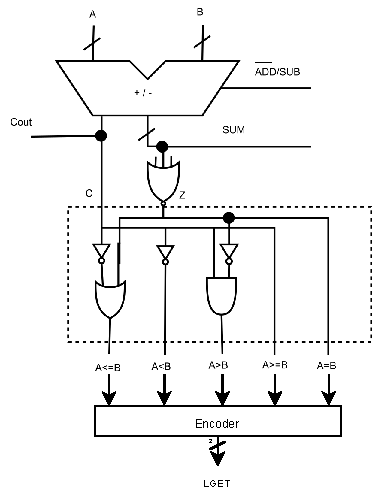
\includegraphics[width=0.3\textwidth]{chapters/4_DecodeStage/images/cmp_final.pdf}
	\caption{Final implementation of the comparator}
	\label{cmp_final}
\end{figure}

\section{Jump and Branch decision}
When taking into consideration jump and branch decision there are many details to exaplin. First, as shown in \autoref{table:decode_instr}, there are some instructions, like JAL and JALR, that need to save the value of the current program counter inside the register R31. For this reason, the value of WS is set to R31 in these king of instructions. 

Another important thing is that when jumping there need to be a change on the program counter. In order to exploit this feature there is a dedicated hardware inside the decode block, that takes into account the computation of the next program counter. All the circuit and its functioning are explained in the next section. 

In the control word there is a dedicated bit for the \texttt{JUMP\_EN}. For the instructions that requires a jump, such as J, JAL, JALR, CALL and RET, this bit is set to 1 by default. For others instruction that may jump, in particular the conditional branches, there is an intermediate step, that is the comparator. In fact, for these instructions, the \texttt{JUMP\_EN} bit is set to 0 by default. Then, thanks to a process inside the control unit, based on the opcode and on the bits of the signal \texttt{LGET}, the \texttt{JUMP\_EN} is set to 1 and the \texttt{IF\_STALL} to 1 as well. This is very important because when jumping, there is the need to wait fetching the next instruction. For this reason the fetch stage is stalled, in order to avoid fetching the next instruction immediately. 

The content of the process that exploit the functionalities just explained is the following:
\newline

\begin{lstlisting}[style=vhdl,caption={VHDL code for the conditional branch},label=conditional_branches_code]
  if (IR_opcode = OP_BEQZ and LGET(0) = '0') then -- BEQZ 
    i_JUMP_EN <= '1';
    IF_STALL <= '1';
  elsif (IR_opcode = OP_BNEZ and LGET(0) = '1') then -- BNEZ
    i_JUMP_EN <= '1';
    IF_STALL <= '1';
  elsif (IR_opcode = OP_BGE and (LGET(1) = '1' or LGET(0) = '0')) then -- BGE
    i_JUMP_EN <= '1';
    IF_STALL <= '1';
  elsif (IR_opcode = OP_BLE and LGET(1) = '0') then -- BLE
    i_JUMP_EN <= '1';
    IF_STALL <= '1';
  elsif (IR_opcode = OP_BGT and LGET = "11") then -- BGT
    i_JUMP_EN <= '1';
    IF_STALL <= '1';
  elsif (IR_opcode = OP_BLT and LGET = "01") then -- BLT
    i_JUMP_EN <= '1';
    IF_STALL <= '1';
  elsif (IR_opcode = OP_CALL and BUSY_WINDOW = '1') then -- CALL
    CALL <= '0';
    i_JUMP_EN <= '0';	
  elsif (IR_opcode = OP_CALL and BUSY_WINDOW = '0' and i_SPILL_delay = '0') then -- CALL
    CALL <= '1';
  elsif (IR_opcode = OP_RET and BUSY_WINDOW = '1') then -- RET
    RET <= '0';
    i_JUMP_EN <= '0';
  end if;
\end{lstlisting}

Looking at the \autoref{tab:lget} we undestand that in order to check a specific branch we have:

\begin{itemize}
  \item BEQZ: if the LSB of \texttt{LGET} is 0, then it means that there is equivalence with 0
  \item BNEZ: if the LSB of \texttt{LGET} is 1, then it means that there is don't have equivalence with 0
  \item BGE: if the LSB of \texttt{LGET} is 0 or if the LSB+1 of \texttt{LGET} is 1
  \item BLE: if the LSB+1 of \texttt{LGET} is 0, then it means that there is less equal
  \item BGT: if LGET = 11
  \item BLT: if LGET = 01
\end{itemize}

The last cases to analyze are the one in which there is CALL or RET. If there is \texttt{BUSY\_WINDOW} equal to 1, it means that the current window is still in use, and so no operation on it have to be executed. In fact \texttt{JUMP\_EN} is set to 0.

The last case is the one when \texttt{BUSY\_WINDOW} and so the execution of the CALL procedure is feasible. In fact, \texttt{CALL} is set to 1.

\section{Next Program Counter computation}
The next program counter computation is included inside the decode block, in order to better manage hazards and jumps. To lighten the load on the ALU, a dedicated P4 adder has been included inside the decode stage to compute the next program counter. 
The full schematic of the decode is shown in \autoref{decode_block}.

\begin{figure}[H]
	\centering
  \addtolength{\leftskip}{-3cm}
  \addtolength{\rightskip}{-3cm}
	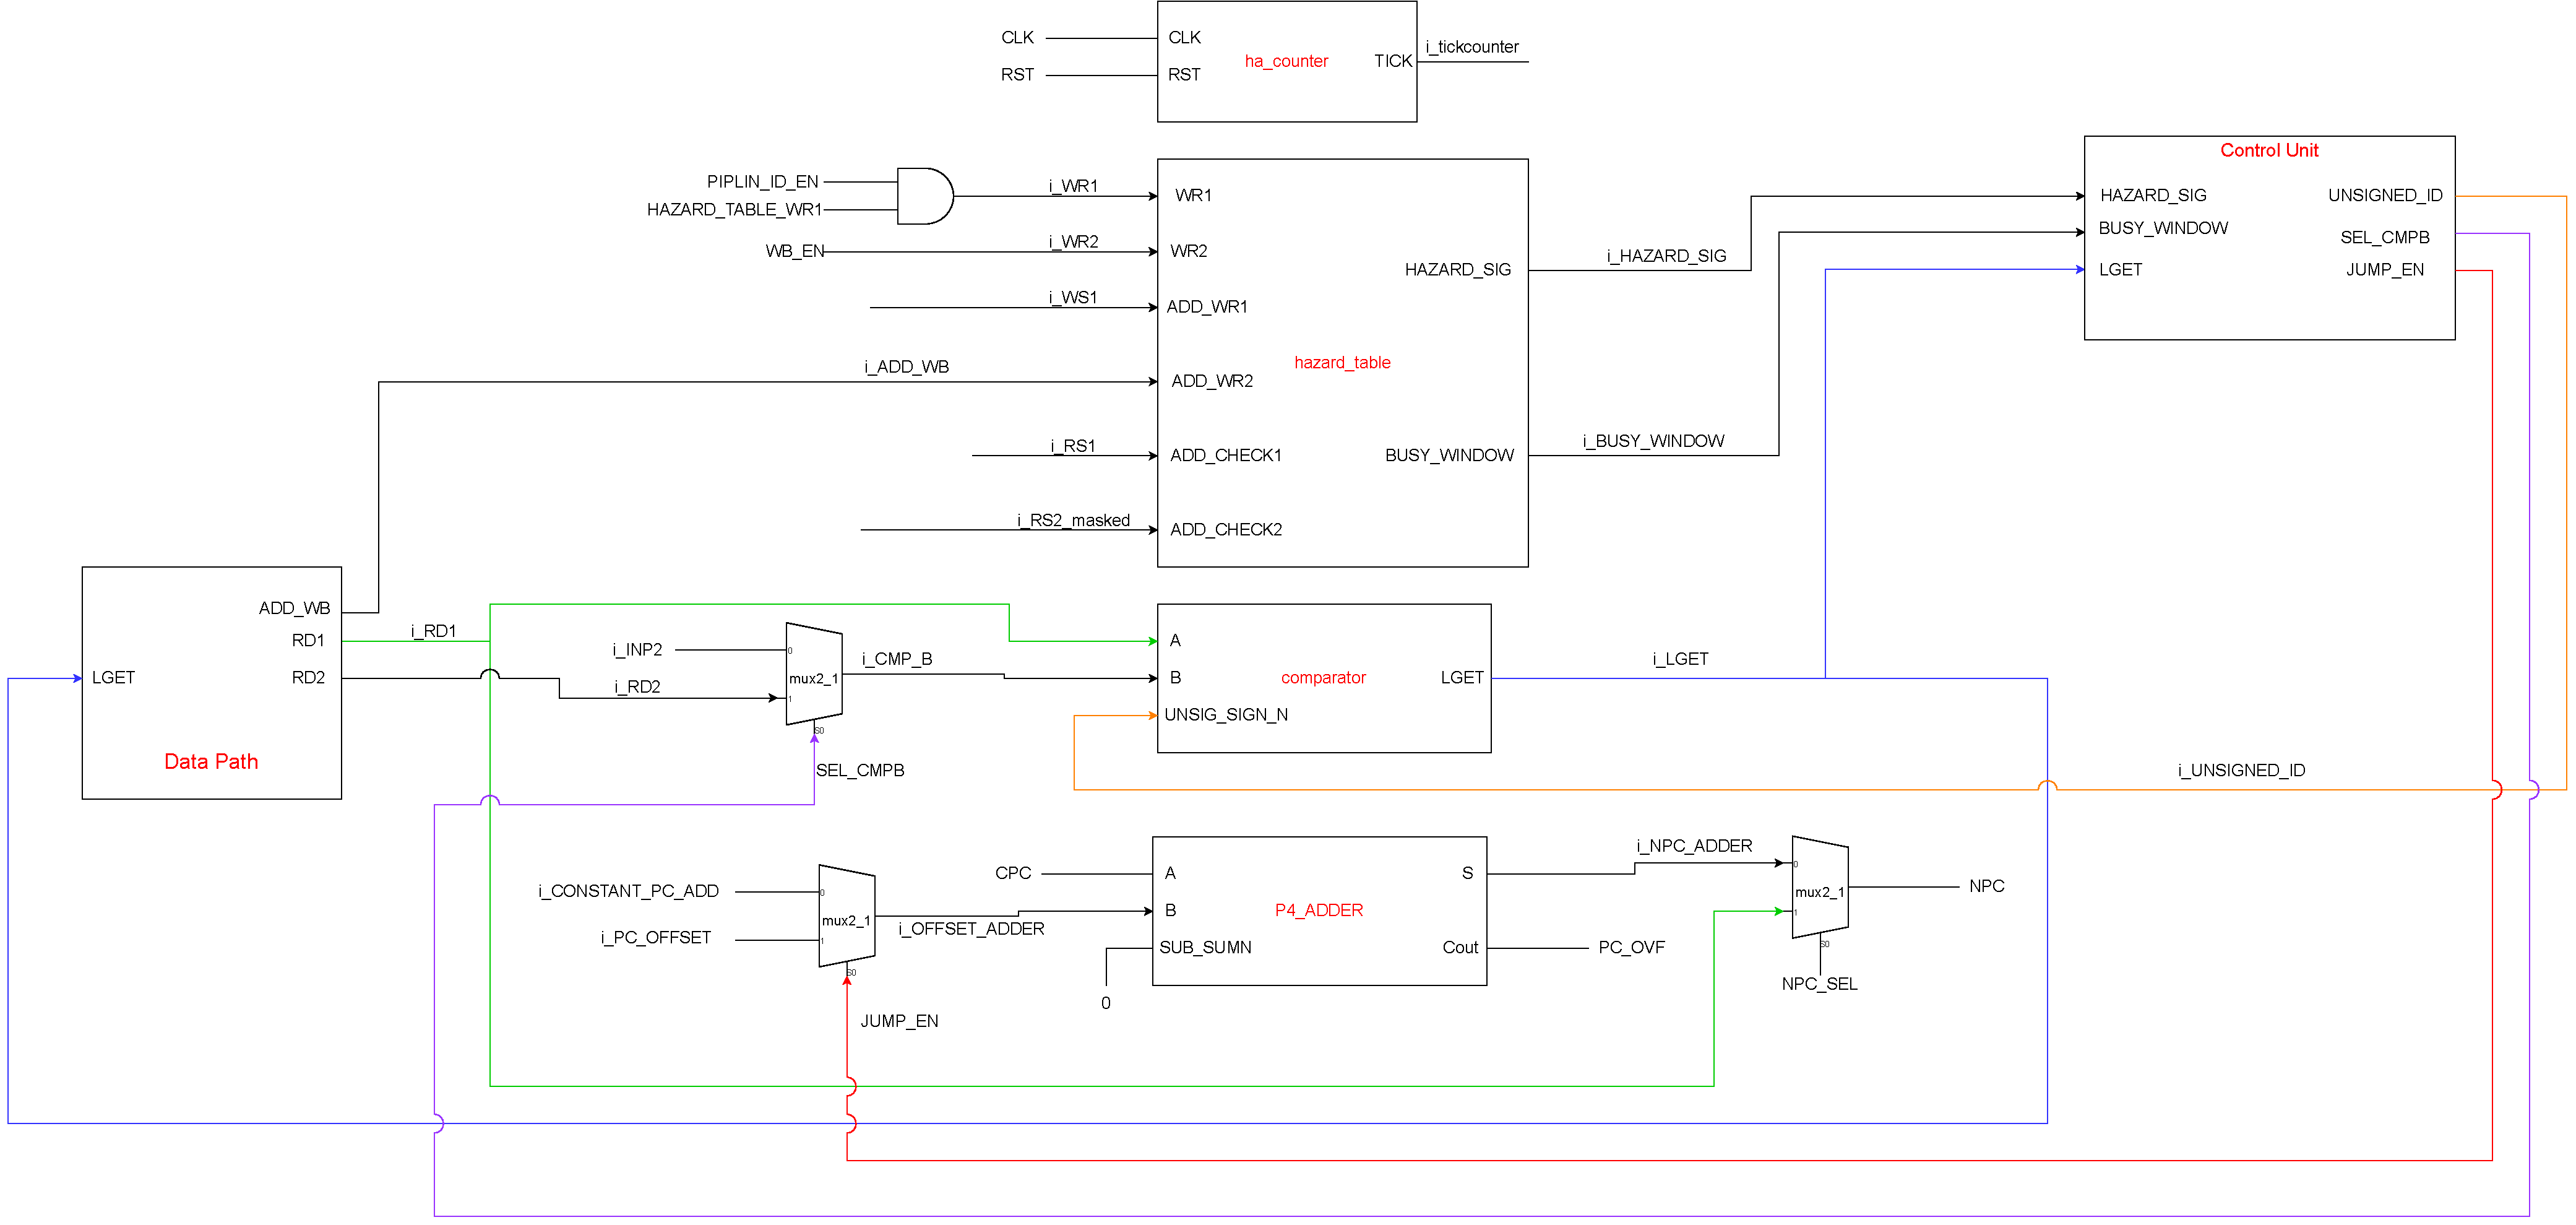
\includegraphics[width=1.2\textwidth]{chapters/4_DecodeStage/images/decode_block.pdf}
	\caption{Schematic of the decode block}
	\label{decode_block}
\end{figure}

There are 2 possible conditions:

\begin{enumerate}
  \item \texttt{JUMP\_EN = 0}: this means that there is no jump. So the program counter should be increased by a constant value, in our case 4. By comparing the explanation and the schematic, it's clear how the left multiplexer, with a 0, will select the signal \texttt{i\_CONSTANT\_PC\_ADD}. Then the two signals enter the P4 Adder and the next program counter is computed. The carry out of the P4 adder is mapped on a signal called \texttt{PC\_OVF}, used to report a program counter overflow. 
  \item \texttt{JUMP\_EN = 1}: this means that there is a jump. So the program counter should be increased by an offset. Looking at the schematic, it's clear how the left multiplexer, with a 1, will select the signal \texttt{i\_PC\_OFFSET}. Then the two signals enter the P4 Adder and the next program counter is computed. 
\end{enumerate}

The multiplexer on the right is controlled by a signal that comes from the control unit, in particular from the control word. The only 3 instructions in which the value of \texttt{NPC\_SEL} is 1, and so it selects RD1, are:

\begin{itemize}
  \item JR
  \item JARL
  \item RET
\end{itemize}

In fact, in these cases, we need to completely change the value of the program counter and put inside it a value read from the register file, in particular \texttt{RD1}.
\section{Tickcounter}
When thinking how to further improve the PRO version of the DLX, an idea was to implement a counter. As it's know, counters are very common inside microprocessors because they are useful keep track of the timing. 
The implementation chosen in the DLX was very simple and straightforward. There is an half-adder on 32 bits that every rising edge of the clock increases the value of the register used inside the tickcounter block to keep track of the value. By doing this we can count the number of ticks and use to estimate the duration of a specific program.
